\capitulo{5}{Aspectos relevantes del desarrollo del proyecto}

\section{Planificación del proyecto}
La planificación del proyecto se ha estructurado en siete fases, las cuales se describen desde la concepción de la idea del proyecto hasta la entrega del final del proyecto. Para visualizar estas tareas se diseño un diagrama de Gantt para entender de mejor manera la distribución del tiempo y la organización de las tareas. A continuación, en la siguiente figura se muestra el diagrama de Gantt del proyecto. 
\begin{figure}[H]
    \centering
    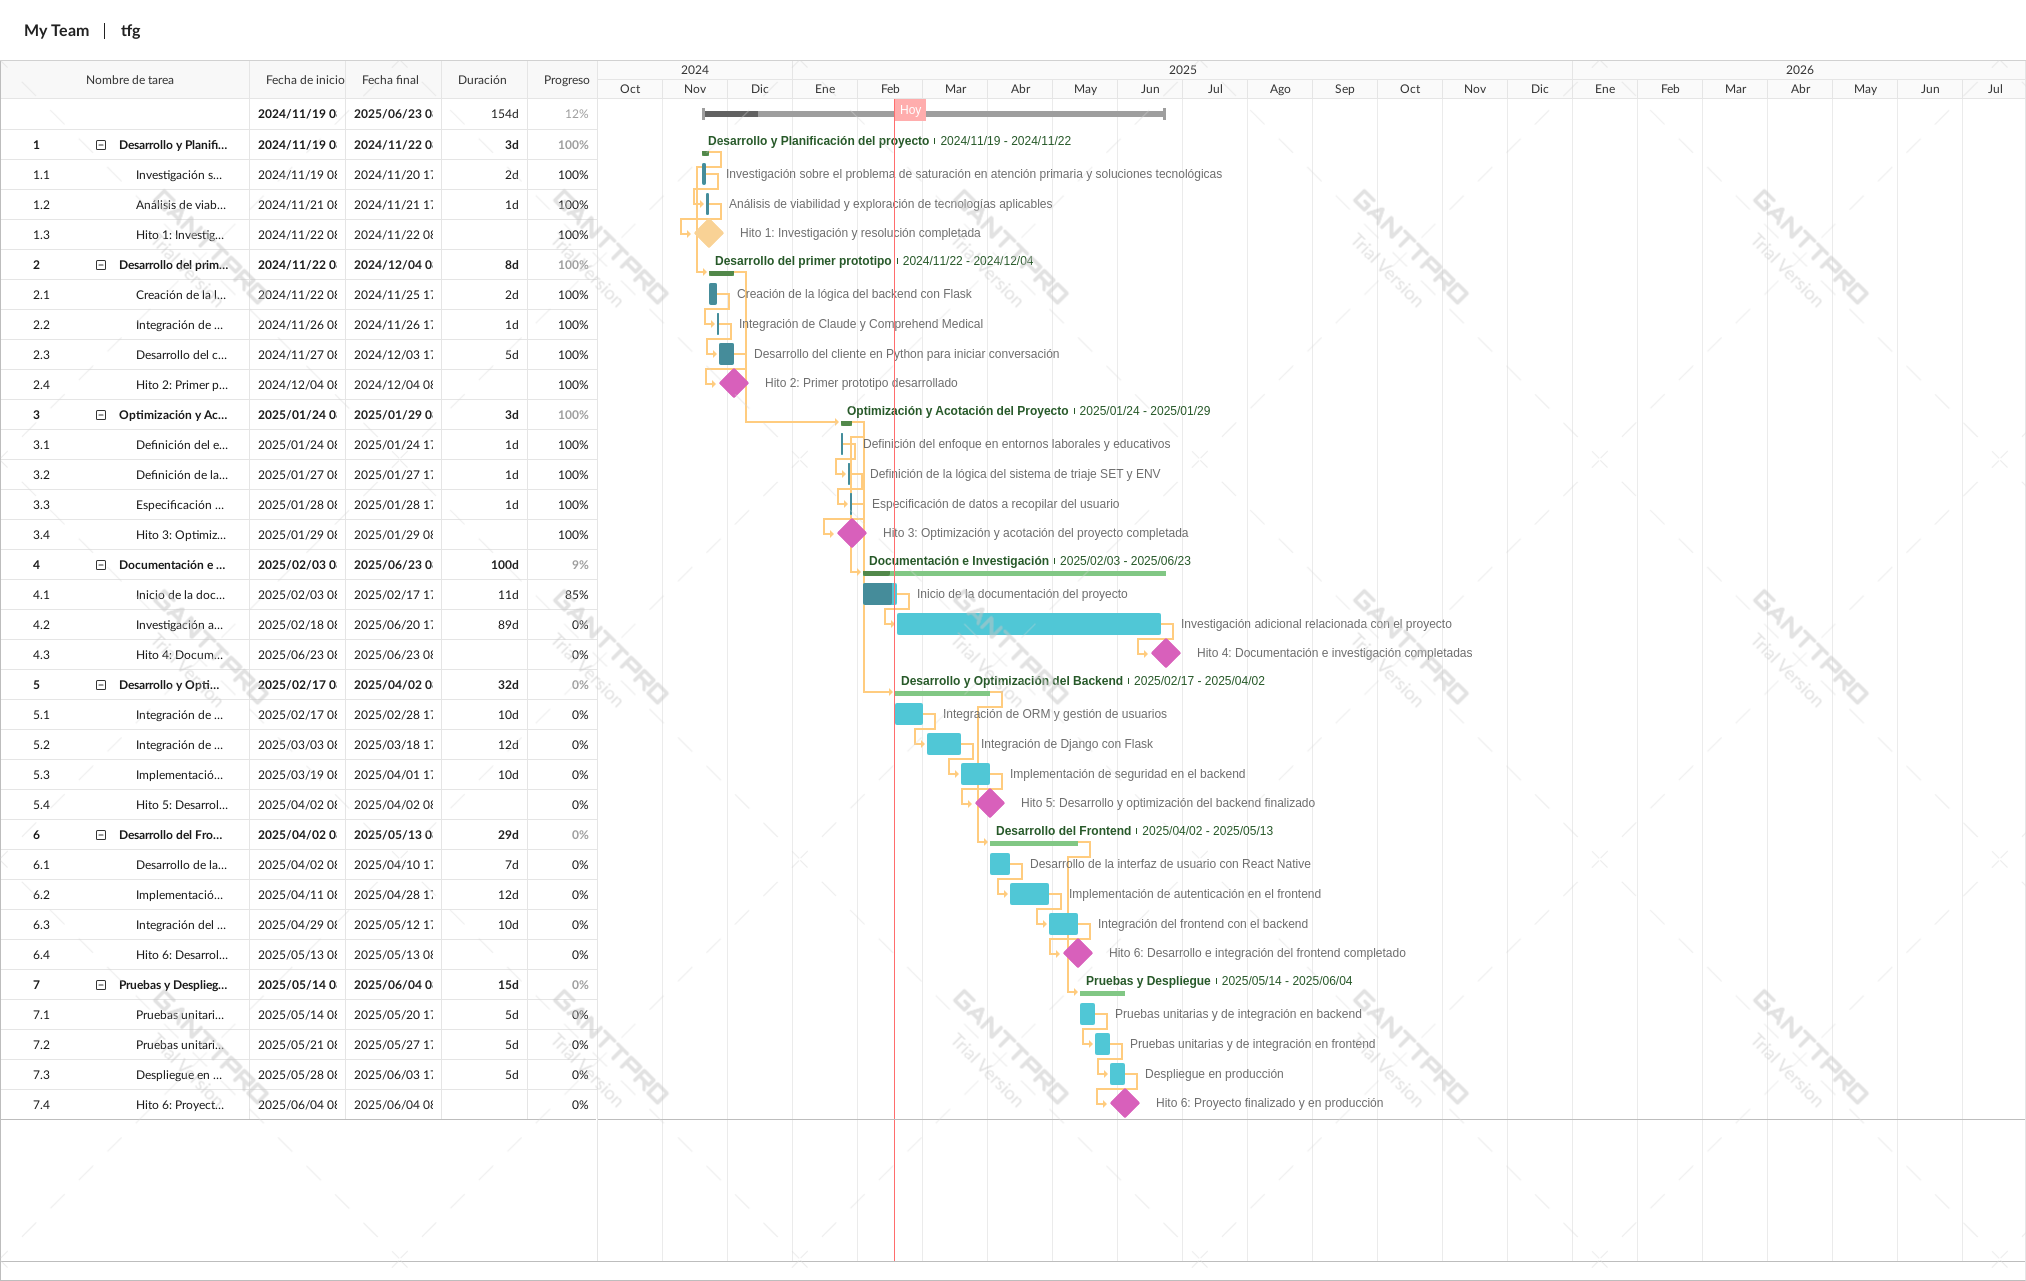
\includegraphics[width=\textwidth]{diagrama-gantt.png}  % Nombre del archivo de la imagen
    \caption{Diagrama de Gantt del proyecto}
    \label{fig:gantt}
\end{figure}

\subsection{Fase 1: Planificación y Desarrollo de la idea}
El proyecto inicio con una fase de investigación y analisis de necesidades. Para ello, se definieron los objetivos generales y específicos, analizando los principales retos tanto técnicos como funcionales. Se optó por utilizar metodologías ágiles para la gestión del desarrollo, facilitando adaptaciones ágiles y eficientes frente a modificaciones en los requerimientos.

En esta fase se realizo un análisis de viabilidad, explorando diversas tecnológias y frameworks para el desarrollo de backend y frontend. Asimismo, se comenzó con la recopilación de datos para establecer la base de conocimiento del chatbot, asegurando su alineación con los objetivos del proyecto.
\subsection{Fase 2: Desarrollo del primer prototipo}
En el primer prototipo del sistema tenía el objetivo de validar la soluciones propuestas en la fase anterior. Se desarrollo una versión minima funcional que incluye:

\begin{itemize}
    \item Se desarrolló un backend en Flask definiendo endpoints para manejar la comunicación con el chatbot y guardar la conversación en un fichero JSON.
    \item Un cliente en Python que consumía la API del backend y permitía al usuario interactuar con el chatbot.
    \item La integración inicial con Amazon Comprehend Medical y Amazon Bedrock con Claude para el procesamiento de lenguaje natural y el análisis de sentimientos.
\end{itemize}

A continuación, se muestra un fragamento del código del backend desarrollado con Flask:

\begin{lstlisting}[language=Python]
    
    